\section{NUTS}

In our current description of the SGHMC algorithm we have the user-defined hyperparameter $L$, the number of steps iterated over before we take a sample. If this number is too small, our samples will be correlated, and hence successive samples would appear to follow a random walk, and we would get slow mixing times. We demonstrate this behaviour by training 3 versions of SGHMC with $L=1,3,5$ (with $\epsilon L$ fixed). The learning curves below show that increasing $L$ increases the speed with which SGHMC reaches low error rates.

\begin{figure}[h!]
\centering
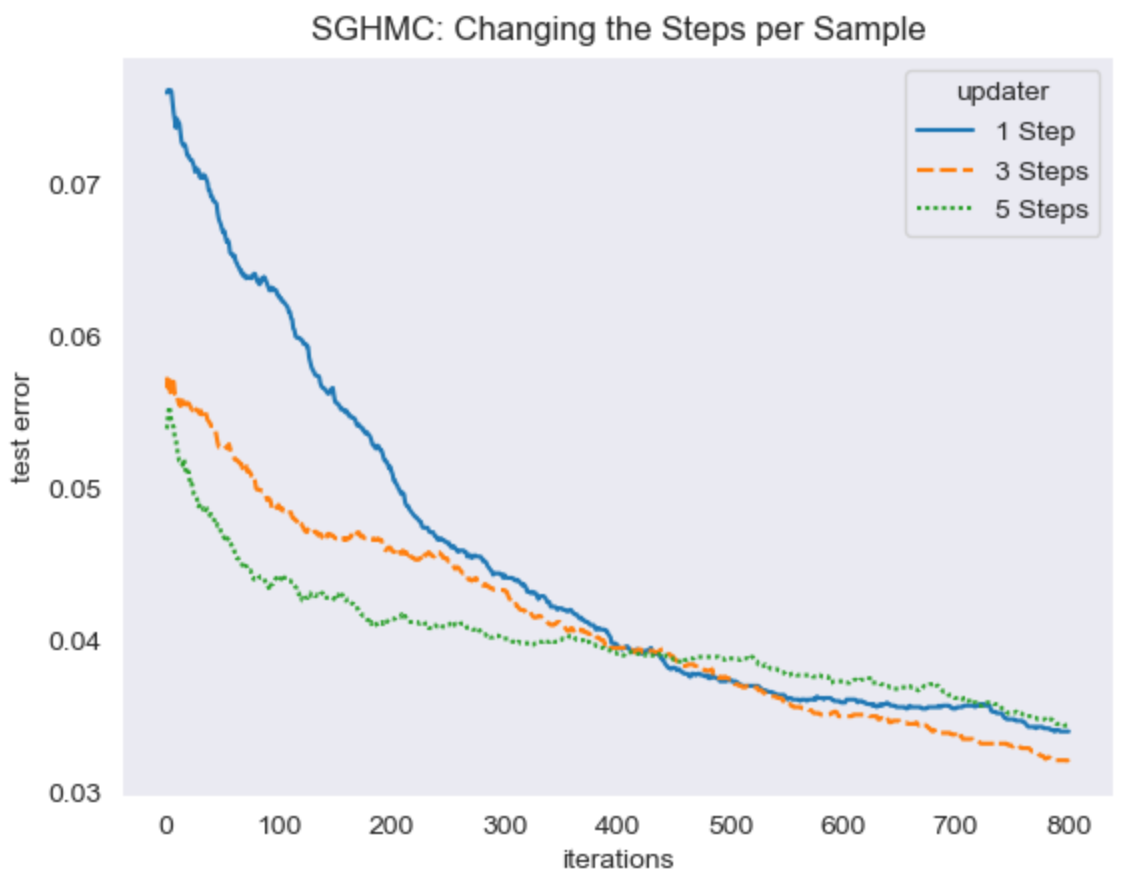
\includegraphics[width=100mm]{parts/Images/changing_num_steps.png}
\caption{Changing the number of steps per sample. Each agent was run for 100 warmup epochs.}
\end{figure}

However, if $L$ is too large we waste computational power, as we continue to step through time even though each sample is already independent of the last. We would like to set $L$ to its optimal value.

Hoffman and Gelman introduce the algorithm NUTS in their paper "The No-U-Turn Sampler: Adaptively Setting Path Lengths in Hamiltonian Monte Carlo" \cite{nuts}. In its basic form this algorithm removes the need for a user to input a value for $L$ in the standard HMC implementation. We converted this NUTS algorithm from being based on HMC to being based on SGHMC, and investigated its power. We will begin by presenting the high level overview of the original NUTS algorithm for HMC sampling.

The key idea is the concept of a 'U-Turn'. This is the point at which the samples of $\theta$ start to get closer to the initial value of $\theta$, rather than away from it. This marks the point at which further steps will likely only waste computational power. Mathematically, for current position $\theta$, initial position $\theta_0$ and momentum $r$, this corresponds to the time at which 

$$ \frac{d}{dt} |\theta - \theta_0|^2 = 2(\theta - \theta_0)\cdot\frac{d\theta}{dt} = 2(\theta - \theta_0)\cdot r< 0$$

where we use the fact that in the dynamics of HMC (and also SGHMC) we have $\frac{d\theta}{dt} = r$. This simple fact suggests an algorithm in which we draw the sample $\theta$ once we have performed enough steps so that $(\theta - \theta_0)\cdot r< 0$. However this is too simplistic an approach - as HMC is an instance of the Metropolis Hastings algorithm we require the Markov Chain of $\theta$ to be reversible, which is not the case here.

To remedy this problem, NUTS requires keeping track of a set $\mathcal{B}$, which contains all values of $(\theta, r)$ as steps are taken both forward and backwards in time. The values at the earliest and latest times considered across a single trajectory are labelled  $(\theta^-, r^-)$ and $(\theta^+, r^+)$ respectively. NUTS starts from a single $(\theta, r)$ and then steps either forward or backwards one step. It then steps forward or backwards 2 steps, then 4 steps, then 8 steps etc until a 'U-Turn' is seen. A description is as follows:

\begin{enumerate}
    \item Start with an initial $(\theta_0, r_0)$
    \item Set $n\leftarrow1$, $\mathcal{B}\leftarrow \{(\theta_0, r_0)\}$, $(\theta^-, r^-) \leftarrow (\theta_0, r_0) $ and $(\theta^+, r^+) \leftarrow (\theta_0, r_0) $ 
 \item While there is no U-Turn at $(\theta^-, r^-)$ nor at $(\theta^+, r^+)$\\ (ie $(\theta^+ - \theta^-)\cdot r^- \geq 0$ and $(\theta^+ - \theta^-)\cdot r^+ \geq 0$): 
 \begin{enumerate}
 \item Choose to go \textit{forwards} or \textit{backwards} in time, each
with probability $\frac{1}{2}$

\item If \textit{forwards}:
\begin{enumerate}
    \item $(\theta, r) \leftarrow (\theta^+, r^+)$

 \item Repeat n times:
 \begin{enumerate}
     \item $(\theta, r) \leftarrow $ Step forward in time from $(\theta, r)$
     \item $\mathcal{B} \leftarrow (\theta, r) \cup \mathcal{B}$
   \end{enumerate}
   \item $(\theta^+, r^+) \leftarrow (\theta, r)$

    \end{enumerate}
    
\item If \textit{backwards}:
\begin{enumerate}
    \item $(\theta, r) \leftarrow (\theta^-, r^-)$

 \item Repeat n times:
 \begin{enumerate}
     \item $(\theta, r) \leftarrow $ Step backwards in time from $(\theta, r)$
     \item $\mathcal{B} \leftarrow (\theta, r) \cup \mathcal{B}$
   \end{enumerate}
   \item $(\theta^-, r^-) \leftarrow (\theta, r)$
   
    \end{enumerate}
    \item $n \leftarrow 2n$
    \end{enumerate}
\item Carefully choose a subset $\mathcal{C} \subseteq \mathcal{B}$. This step is the key to the Markov Chain being reversible, however for clarity's sake we will not go into detail as to how this is done here.
\item Sample an element of $\mathcal{C}$

    \end{enumerate}



The benefit to this algorithm is that it removes the need to set the number of steps performed before we sample, as we keep stepping until a 'U-Turn' is seen. We should note here that in the original form of NUTS, the 'step' being referred to in $3biiA$ and $3ciiA$ is the step of the HMC algorithm. We edited the NUTS Pyro source code to make it perform SGHMC steps, and we named this SGNUTS.

There were some doubts as to whether the NUTS algorithm would work when using SGHMC steps instead of HMC steps. This was because NUTS requires the ability to step backwards in time, while an SGHMC step includes an injection of stochastic noise. As there is no action that undoes this injection, there was a worry that the backwards step through time in NUTS would become a problem. We explain how we attempted to solve this problem at the end of the next section.

\subsection{Implementation of SGNUTS}
To build SGNUTS we started with the Pyro source code for NUTS \cite{nuts_code} which takes the Pyro HMC class as its parent. We altered this to instead inherit from our SGHMC class. This required removing step-size adaptation and mass matrix adaptation functionality from NUTS, as our implementation of SGHMC was not able to interface with this. It also required introducing some caching methods into the SGHMC class - to help keep things simple in our original SGHMC class we did this in a new class, named SGHMC\_for\_NUTS. Most importantly, we had to alter the $(\theta,v)$ step update rule which is hardcoded in NUTS. This meant that instead of being the HMC update step it was now the SGHMC update step of:

$$
    \theta \leftarrow 
    \begin{cases}\theta + \epsilon M^{-1}r, & \text{{\textit{forwards step}}}\\
                \theta - \epsilon M^{-1}r,  & \text{{\textit{backwards step}}}

\end{cases}
$$
$$
    r \leftarrow 
    \begin{cases}
                
    r - \epsilon \nabla \tilde{U}(\theta) - \epsilon C M^{-1}r + \mathcal{N}(0,2(C-\hat{B})\epsilon), & \text{{\textit{forwards step}}}\\
   
    r + \epsilon \nabla \tilde{U}(\theta) - \epsilon C M^{-1}r + \mathcal{N}(0,2(C-\hat{B})\epsilon), & \text{{\textit{backwards step}}}\\
 \end{cases}
    $$

In particular, note that there is an injection of stochastic noise and momentum-reducing friction in both the forward steps and the backward steps. This is not ideal, as our backwards step in time does not undo a forward step, which likely breaks the reversibility of the Markov Chain being considered in NUTS. However we investigated this nonetheless.

\subsection{Results} 

We tested the SGNUTS algorithm on the BNNs described earlier. We ran SGNUTS for only 20 warmup epoch and 50 epochs as the code was slower than SGHMC to run. The learning curves were as follows:

\begin{figure}[h!]
\centering
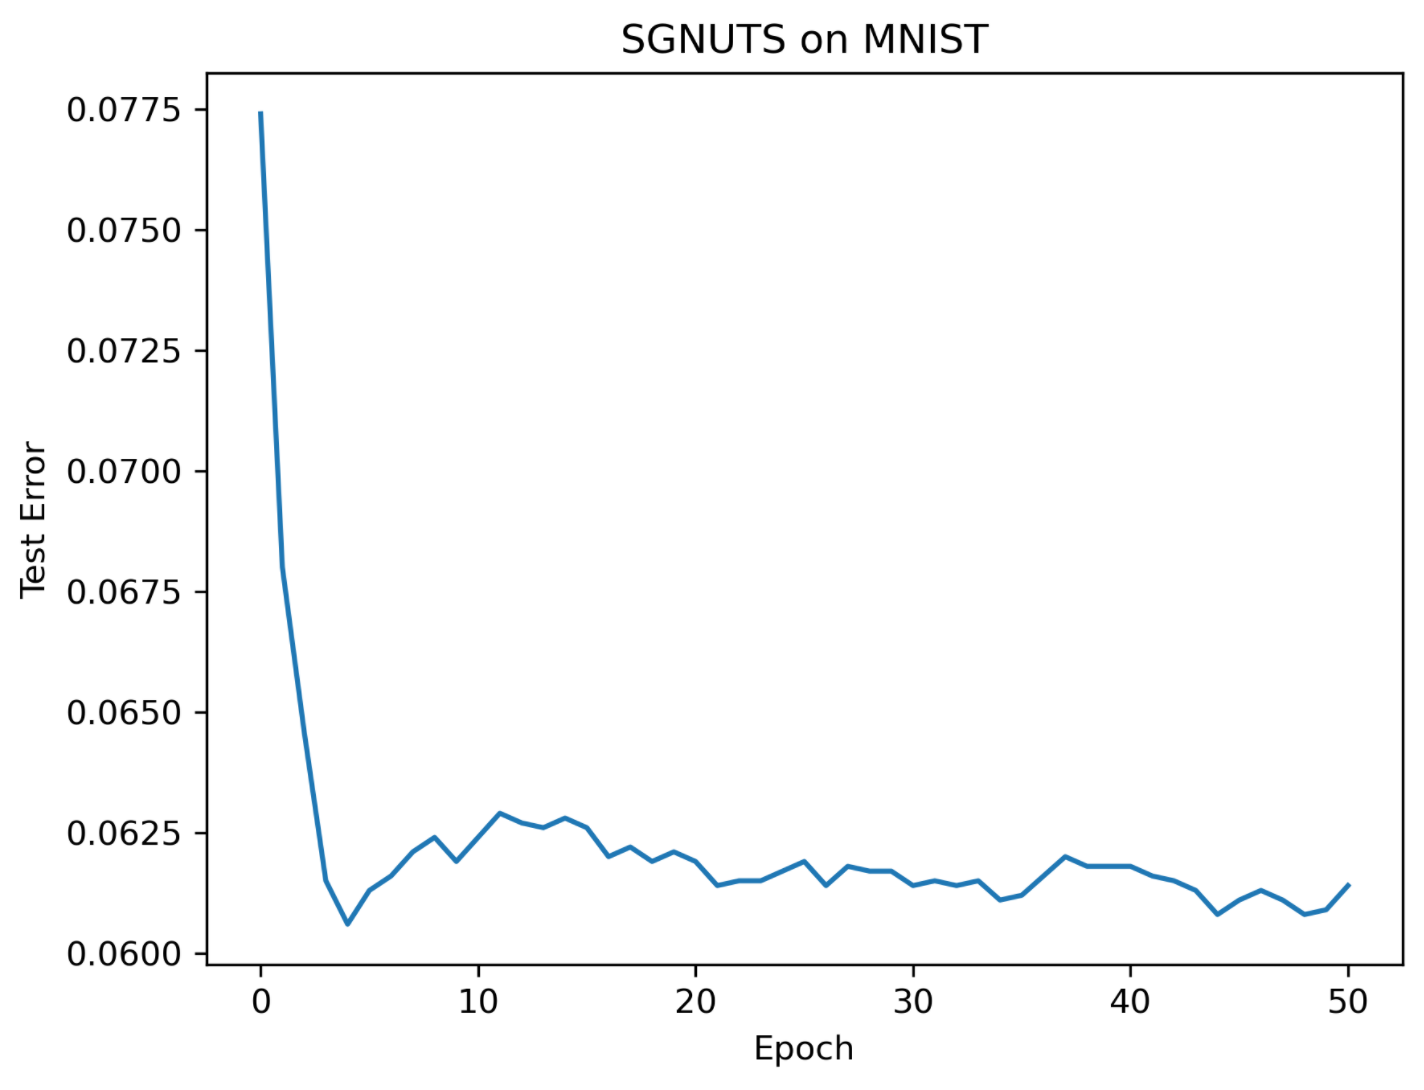
\includegraphics[width=70mm]{parts/Images/SGNUTS_MNIST.png}
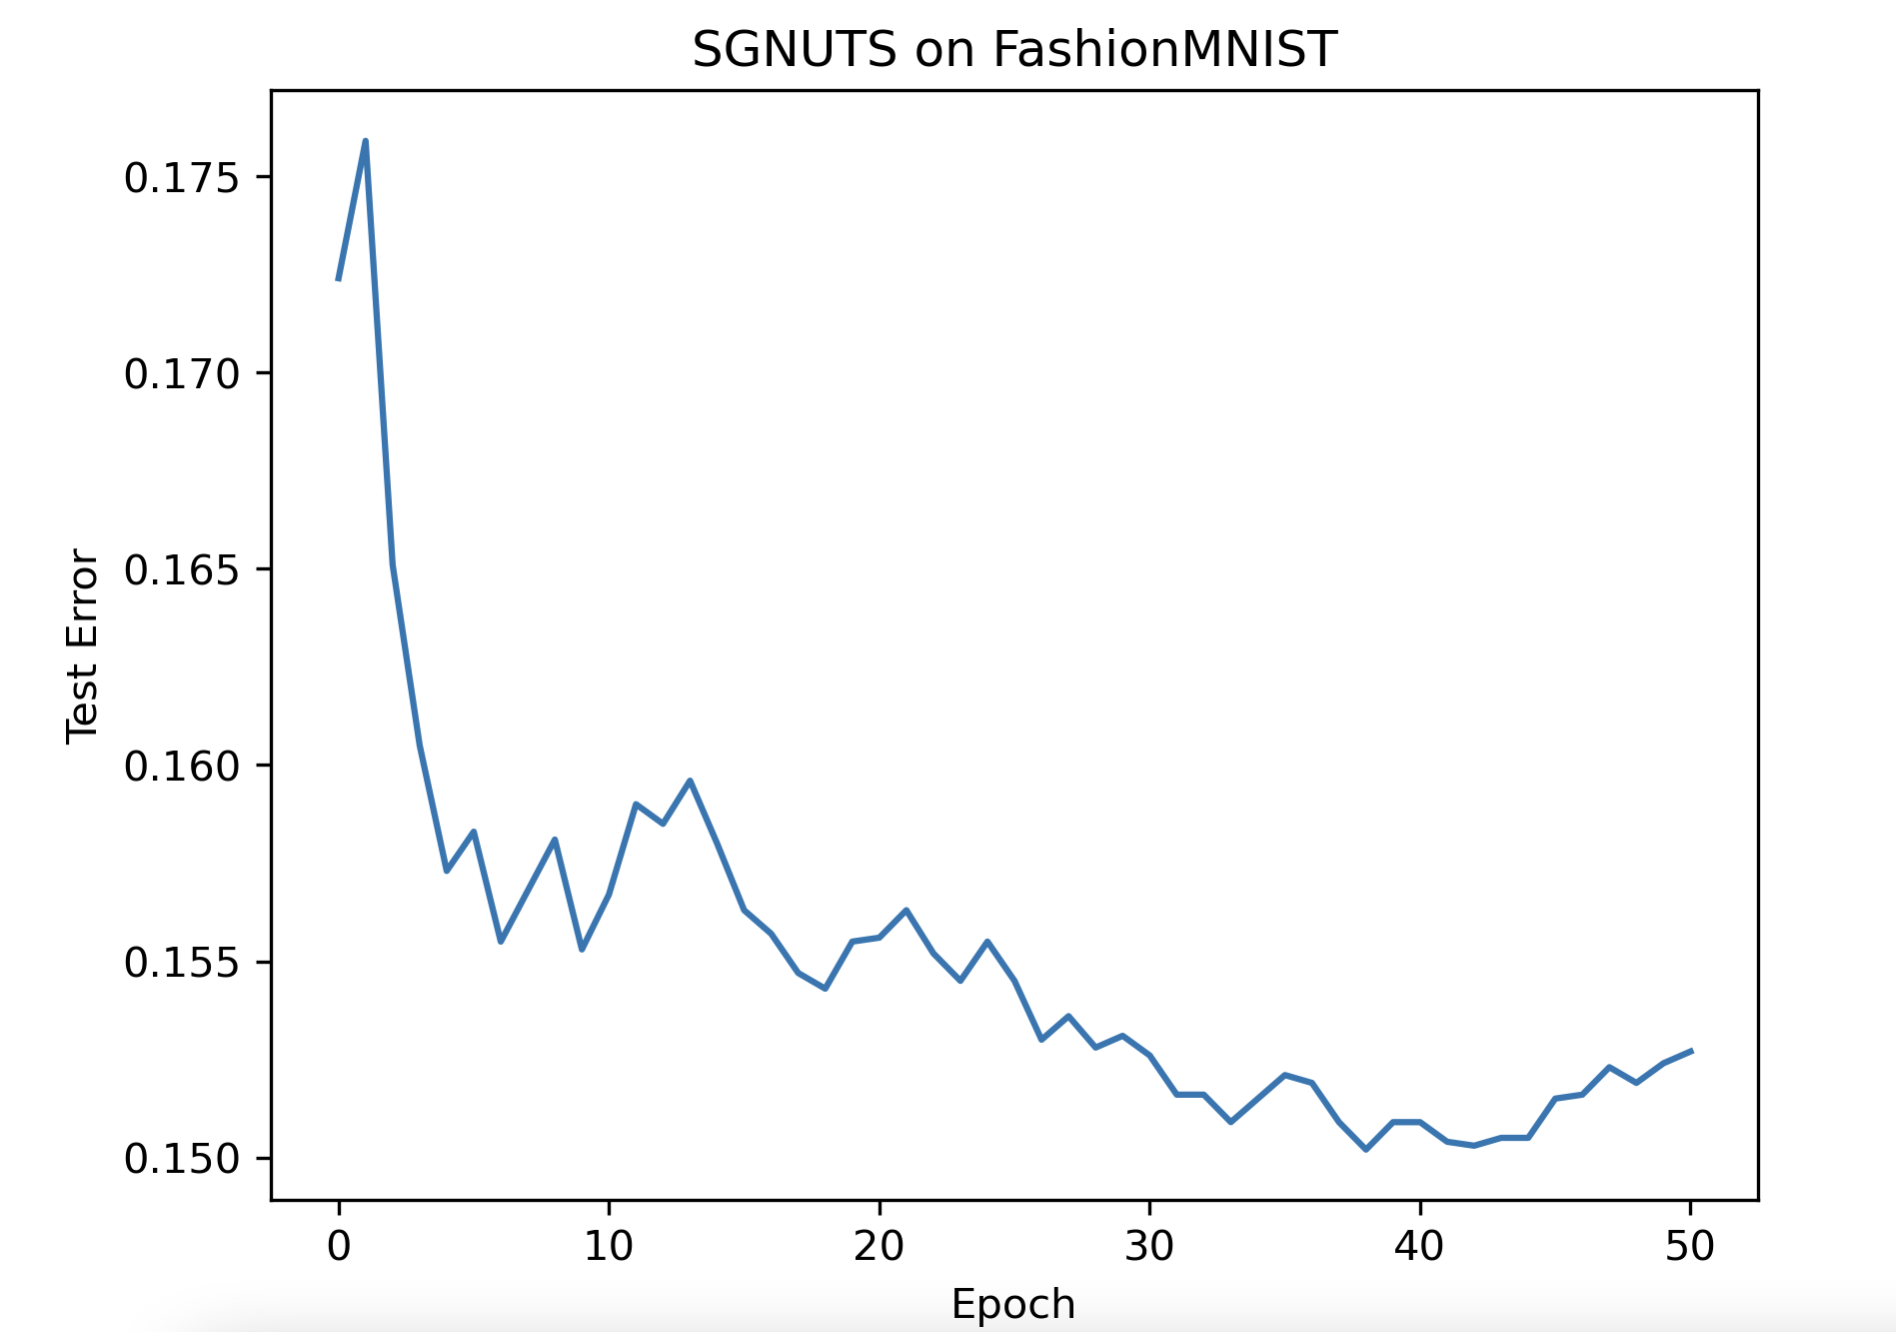
\includegraphics[width=75mm]{parts/Images/SGNUTS_Fashion.png}
\caption{Classifying MNIST and FashionMNIST with SGNUTS}
\end{figure}

The final accuracies were 0.94 for MNIST and 0.85 for FashionMNIST which are similar to the accuracies obtained using SGNUTS (0.97 and 0.86 respectively). This accuracy demonstrates that there is convergence to the true posterior in SGNUTS. This suggests that, like SGHMC itself, the SGNUTS Markov Chain is likely reversible in some (non traditional) sense. Denoting the posterior as $\pi(\theta, r)$, and transition kernels as $P(\theta, r| \theta', r')$, it is shown in (\cite{sghmc}) that SGHMC satisfies
$$ \pi(\theta,r)P_{SGHMC}(\theta,r|\theta',r') = \pi(\theta',-r')P_{SGHMC}(\theta',-r'|\theta,-r)$$

and it is suggested that this is the reason why the SGHMC algorithm works, despite not being reversible in the traditional sense. It would be interesting to consider if a similar property holds for $P_{SGNUTS}$.

While accurate, SGNUTS is slower to run than SGHMC to produce a single sample. It does however reach relatively high accuracies in a short amount of time. We measured the accuracy after the first epoch of SGHMC and NUTS as we changed the number of warmup epochs, and we measured how long they took to train.

\begin{center}
\begin{tabular}{ccccc} 
\hline
Number of Warmup-Epochs &\multicolumn{2}{c}{SGHMC}& \multicolumn{2}{c}{SGNUTS} \\
& Accuracy & Time (s) & Accuracy & Time (s) \\
 \hline
 0 &0.7747  &  3.2&0.8715&28.3\\ 
 1 & 0.5764 & 4.5 &0.9296&127.2\\ 
 2 & 0.4141 & 6.2&0.9231&453.3\\ 
 5 &0.6471& 11.4 &&\\ 
 10 &0.7100& 20.3 &&\\ 
 25 &0.8866& 50.2 &&\\ 
 \hline
\end{tabular}
\end{center}

In particular, SGNUTS reached an accuracy of 0.87 in 28s, while SGHMC reached 0.89 in 50s. This suggests a new algorithm that uses both SGNUTS and SGHMC - we could run a single epoch of SGNUTS so that we quickly approach the posterior distribution, at which point we switch to running SGHMC. It should be noted the speed up suggested by the above results would only be 30s seconds, however maybe on more complex datasets this could be larger. It would be interesting to investigate this if we had more time.